\documentclass[11pt,preprint, authoryear]{elsarticle}

\usepackage{lmodern}
%%%% My spacing
\usepackage{setspace}
\setstretch{1.2}
\DeclareMathSizes{12}{14}{10}{10}

% Wrap around which gives all figures included the [H] command, or places it "here". This can be tedious to code in Rmarkdown.
\usepackage{float}
\let\origfigure\figure
\let\endorigfigure\endfigure
\renewenvironment{figure}[1][2] {
    \expandafter\origfigure\expandafter[H]
} {
    \endorigfigure
}

\let\origtable\table
\let\endorigtable\endtable
\renewenvironment{table}[1][2] {
    \expandafter\origtable\expandafter[H]
} {
    \endorigtable
}


\usepackage{ifxetex,ifluatex}
\usepackage{fixltx2e} % provides \textsubscript
\ifnum 0\ifxetex 1\fi\ifluatex 1\fi=0 % if pdftex
  \usepackage[T1]{fontenc}
  \usepackage[utf8]{inputenc}
\else % if luatex or xelatex
  \ifxetex
    \usepackage{mathspec}
    \usepackage{xltxtra,xunicode}
  \else
    \usepackage{fontspec}
  \fi
  \defaultfontfeatures{Mapping=tex-text,Scale=MatchLowercase}
  \newcommand{\euro}{€}
\fi

\usepackage{amssymb, amsmath, amsthm, amsfonts}

\def\bibsection{\section*{References}} %%% Make "References" appear before bibliography


\usepackage[round]{natbib}

\usepackage{longtable}
\usepackage[margin=2.3cm,bottom=2cm,top=2.5cm, includefoot]{geometry}
\usepackage{fancyhdr}
\usepackage[bottom, hang, flushmargin]{footmisc}
\usepackage{graphicx}
\numberwithin{equation}{section}
\numberwithin{figure}{section}
\numberwithin{table}{section}
\setlength{\parindent}{0cm}
\setlength{\parskip}{1.3ex plus 0.5ex minus 0.3ex}
\usepackage{textcomp}
\renewcommand{\headrulewidth}{0.2pt}
\renewcommand{\footrulewidth}{0.3pt}

\usepackage{array}
\newcolumntype{x}[1]{>{\centering\arraybackslash\hspace{0pt}}p{#1}}

%%%%  Remove the "preprint submitted to" part. Don't worry about this either, it just looks better without it:
\makeatletter
\def\ps@pprintTitle{%
  \let\@oddhead\@empty
  \let\@evenhead\@empty
  \let\@oddfoot\@empty
  \let\@evenfoot\@oddfoot
}
\makeatother

 \def\tightlist{} % This allows for subbullets!

\usepackage{hyperref}
\hypersetup{breaklinks=true,
            bookmarks=true,
            colorlinks=true,
            citecolor=blue,
            urlcolor=blue,
            linkcolor=blue,
            pdfborder={0 0 0}}


% The following packages allow huxtable to work:
\usepackage{siunitx}
\usepackage{multirow}
\usepackage{hhline}
\usepackage{calc}
\usepackage{tabularx}
\usepackage{booktabs}
\usepackage{caption}


\newenvironment{columns}[1][]{}{}

\newenvironment{column}[1]{\begin{minipage}{#1}\ignorespaces}{%
\end{minipage}
\ifhmode\unskip\fi
\aftergroup\useignorespacesandallpars}

\def\useignorespacesandallpars#1\ignorespaces\fi{%
#1\fi\ignorespacesandallpars}

\makeatletter
\def\ignorespacesandallpars{%
  \@ifnextchar\par
    {\expandafter\ignorespacesandallpars\@gobble}%
    {}%
}
\makeatother

\newenvironment{CSLReferences}[2]{%
}

\urlstyle{same}  % don't use monospace font for urls
\setlength{\parindent}{0pt}
\setlength{\parskip}{6pt plus 2pt minus 1pt}
\setlength{\emergencystretch}{3em}  % prevent overfull lines
\setcounter{secnumdepth}{5}

%%% Use protect on footnotes to avoid problems with footnotes in titles
\let\rmarkdownfootnote\footnote%
\def\footnote{\protect\rmarkdownfootnote}
\IfFileExists{upquote.sty}{\usepackage{upquote}}{}

%%% Include extra packages specified by user

%%% Hard setting column skips for reports - this ensures greater consistency and control over the length settings in the document.
%% page layout
%% paragraphs
\setlength{\baselineskip}{12pt plus 0pt minus 0pt}
\setlength{\parskip}{12pt plus 0pt minus 0pt}
\setlength{\parindent}{0pt plus 0pt minus 0pt}
%% floats
\setlength{\floatsep}{12pt plus 0 pt minus 0pt}
\setlength{\textfloatsep}{20pt plus 0pt minus 0pt}
\setlength{\intextsep}{14pt plus 0pt minus 0pt}
\setlength{\dbltextfloatsep}{20pt plus 0pt minus 0pt}
\setlength{\dblfloatsep}{14pt plus 0pt minus 0pt}
%% maths
\setlength{\abovedisplayskip}{12pt plus 0pt minus 0pt}
\setlength{\belowdisplayskip}{12pt plus 0pt minus 0pt}
%% lists
\setlength{\topsep}{10pt plus 0pt minus 0pt}
\setlength{\partopsep}{3pt plus 0pt minus 0pt}
\setlength{\itemsep}{5pt plus 0pt minus 0pt}
\setlength{\labelsep}{8mm plus 0mm minus 0mm}
\setlength{\parsep}{\the\parskip}
\setlength{\listparindent}{\the\parindent}
%% verbatim
\setlength{\fboxsep}{5pt plus 0pt minus 0pt}



\begin{document}



\begin{frontmatter}  %

\title{Insights Into the History of the Olympic Games}

% Set to FALSE if wanting to remove title (for submission)




\author[Add1]{Anna Mayer}
\ead{28776534@sun.ac.za}





\address[Add1]{Stellenbosch Unviersity}


\begin{abstract}
\small{
With the upcoming Summer Olympics in Paris, who is not interested in
having a closer look into the history of summer but also winter Olympics
and the different success stories of athletes, countries and
specifically India.
}
\end{abstract}

\vspace{1cm}


\begin{keyword}
\footnotesize{
Olympics \sep Summer \sep Winter \\
\vspace{0.3cm}
}
\end{keyword}



\vspace{0.5cm}

\end{frontmatter}

\setcounter{footnote}{0}



%________________________
% Header and Footers
%%%%%%%%%%%%%%%%%%%%%%%%%%%%%%%%%
\pagestyle{fancy}
\chead{}
\rhead{}
\lfoot{}
\rfoot{\footnotesize Page \thepage}
\lhead{}
%\rfoot{\footnotesize Page \thepage } % "e.g. Page 2"
\cfoot{}

%\setlength\headheight{30pt}
%%%%%%%%%%%%%%%%%%%%%%%%%%%%%%%%%
%________________________

\headsep 35pt % So that header does not go over title




\hypertarget{introduction}{%
\section{\texorpdfstring{Introduction
\label{Introduction}}{Introduction }}\label{introduction}}

With the upcoming Summer Olympics starting on July 26 in Paris, France,
the general interst is rising again with regards to past Olympics,
trends and the greatest athletes of all times. This news report will dig
deeper into past Summer and Winter Olympics and analyse the performance
of different countries, with particular focus on India and their
successes. To keep it as brief and accessible as possible, the main part
of this news report will be in bullet points.

\hypertarget{data}{%
\section{Data}\label{data}}

\begin{itemize}
\tightlist
\item
  The data used for this analysis is threefold:

  \begin{itemize}
  \tightlist
  \item
    Data on Winter Olympic Games
  \item
    Data on Summer Olympic Games
  \item
    General GDP and population size data
  \end{itemize}
\end{itemize}

\hypertarget{analysis}{%
\section{Analysis}\label{analysis}}

\hypertarget{indias-performance-compared-to-other-countries}{%
\subsection{India's performance compared to other
countries}\label{indias-performance-compared-to-other-countries}}

\begin{itemize}
\item
  India's performance in past summer Olympics compared to similarly
  sized economies (including South America)

  \begin{itemize}
  \tightlist
  \item
    Chose countries with relatively similar GDP per Capita that also
    participated in past Summer Olympics
  \item
    Countries from South America: For example: Colombia
  \end{itemize}
\end{itemize}

\begin{figure}[H]

{\centering \includegraphics{Question4_files/figure-latex/Figure1-1} 

}

\caption{Medals Table for Emerging Country over Time \label{Figure1}}\label{fig:Figure1}
\end{figure}

\begin{itemize}
\tightlist
\item
  Potential explanation for India's performance over time:

  \begin{itemize}
  \tightlist
  \item
    Main medals won in Hockey
  \item
    Only assigned one medal for the whole team for a medal won in a team
    sport discipline during the Olympics
  \end{itemize}
\end{itemize}

\hypertarget{dominant-countries-in-summer-olympics-over-time}{%
\subsection{Dominant countries in Summer Olympics over
time}\label{dominant-countries-in-summer-olympics-over-time}}

\begin{figure}[H]

{\centering 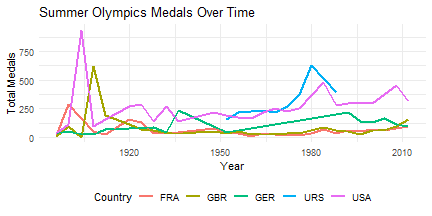
\includegraphics{Question4_files/figure-latex/Figure2-1} 

}

\caption{Top Countries Summer Olympics \label{Figure2}}\label{fig:Figure2}
\end{figure}

\begin{itemize}
\tightlist
\item
  US generally strong over time in Summer Olympics
\item
  Former Soviet Union also tended to be strong in Summer Olympics
\end{itemize}

\hypertarget{dominant-countries-in-winter-olympics-over-time}{%
\subsection{Dominant countries in Winter Olympics over
time}\label{dominant-countries-in-winter-olympics-over-time}}

\begin{figure}[H]

{\centering \includegraphics{Question4_files/figure-latex/Figure3-1} 

}

\caption{Top Countries Winter Olympics \label{Figure3}}\label{fig:Figure3}
\end{figure}

\begin{itemize}
\tightlist
\item
  US generally also strong in Winter Olympics
\item
  Generally northern countries with snow/ mountains more successful
  (which intuitively makes sense)
\item
  Former Soviet Union was also strong in Winter Olympics. Logically not
  anymore today, as it does not exist anymore.
\item
  Note that in the last two graphs there might be a bias, as I could not
  account for all the team sports in the data
\end{itemize}

\hypertarget{gold-per-capita-summer-olympics}{%
\subsection{Gold per Capita Summer
Olympics}\label{gold-per-capita-summer-olympics}}

\begin{figure}[H]

{\centering 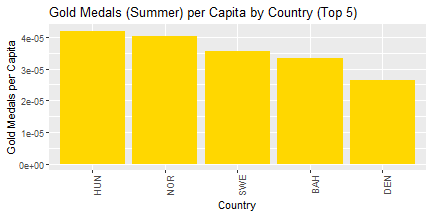
\includegraphics{Question4_files/figure-latex/Figure4-1} 

}

\caption{Gold per Capita Summer Olympics \label{Figure4}}\label{fig:Figure4}
\end{figure}

\begin{itemize}
\tightlist
\item
  Hungary most gold medals per Capita

  \begin{itemize}
  \tightlist
  \item
    Followed by countries that as well do not have a big population
    which explains the result compared to for example the US
  \end{itemize}
\end{itemize}

\hypertarget{gold-per-capita-winter-olympics}{%
\subsection{Gold per Capita Winter
Olympics}\label{gold-per-capita-winter-olympics}}

\begin{figure}[H]

{\centering 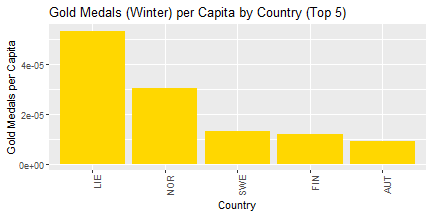
\includegraphics{Question4_files/figure-latex/Figure5-1} 

}

\caption{Gold per Capita Winter Olympics \label{Figure5}}\label{fig:Figure5}
\end{figure}

\begin{itemize}
\tightlist
\item
  Interestingly Liechtenstein most gold medals per Capita

  \begin{itemize}
  \tightlist
  \item
    But makes sense as not a lot of inhabitants
  \item
    Countries that follow also not extremely populated and countries
    that have mountains/ can do winter sports
  \end{itemize}
\end{itemize}

\hypertarget{personal-favourite-sport---slalom-alpine-skiing-winter-olympics}{%
\subsection{Personal Favourite Sport - Slalom Alpine Skiing (Winter
Olympics)}\label{personal-favourite-sport---slalom-alpine-skiing-winter-olympics}}

\begin{itemize}
\tightlist
\item
  Bar plot showing the top 10 athletes in Slalom Alpine Skiing by the
  total amount of medals they got over time
\end{itemize}

\begin{figure}[H]

{\centering 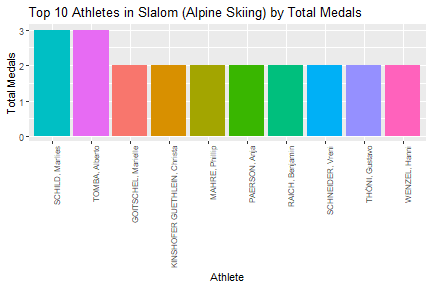
\includegraphics{Question4_files/figure-latex/Figure6-1} 

}

\caption{Top Athletes Slalom \label{Figure6}}\label{fig:Figure6}
\end{figure}

\begin{itemize}
\tightlist
\item
  Marlies Schild and Alberto Tomba both best athletes

  \begin{itemize}
  \tightlist
  \item
    Only focusing on Slalom within Alpine Skiing; explains why maximum
    of medals is 3 per athlete
  \end{itemize}
\end{itemize}

\hypertarget{conclusion}{%
\section{Conclusion}\label{conclusion}}

This report has hopefully helped to get you excited about the upcoming
Summer and hopefully soon to be Winter Olympics, and to remind you of
some of the historical figures in different disciplines within the
Olympics and the performance of countries.

\bibliography{Tex/ref}





\end{document}
